%!TEX root = ../Project.tex

\subsection{Allocation algorithm}

% Writeup from the meeting with JC

% [@todo nice and modular]
% [@todo list constraints mathematically]

\subsubsection{Human aspects}
\label{sec:algo_humanaspects}

During the research period, discussions with academic and administrative staff
in both pilot departments revealed that the current method of module
allocation is not particularly complex. With several hundred students in the
History department, it is impossible for a human to do a uniformly ``fair''
job of allocating modules to students. The staff simply try their best to
allocate as many high choices as possible.

For example, the History department allocates between one and four modules to
each of their students. The administrators and academic staff recounted how,
during the allocation period, every surface in departmental offices would be
covered with sheets of paper (one per student, numbering almost one
thousand in total) on which students had ranked their modules. The departments
would attempt to perform the best allocation possible, though clearly they had
no way of verifying mathematically that the allocation was optimal.

With this information in hand, I began to investigate how the departments and
students saw each of the choices. This influences how what the aim of the
solver will be. One could imagine an imaginary score function that a staff
member might have in their head while allocating modules:

\begin{itemize}
  \item A first choice is perfect -- if every student received every one of
        their first choices, they could not complain about the allocation.
  \item A second or third choice is alright -- a student would not be too
        displeased to be taking their second or third choice module.
  \item A fourth or fifth choice should be avoided where possible, but is not
        a show-stopper.
  \item One would expect a student who was being made to take their sixth or
        lower choice to be fairly unhappy.
\end{itemize}

Mathematically, one could sum a score for each allocation as follows:

$$
c_1(x_1) + c_2(x_2) + c_3(x_3) ...
$$

...where $x_i$ is the number of $i^{th}$ choices that that allocation created.
The coefficient multiplied by the number of $i^{th}$ choices indicates a
penalty applied by the system -- this penalty increases depending on how
negative that choice is deemed to be.

While not particularly complex, instructing the solver to minimise this result
would maximise the number of highly ranked choices. This forms the basis for
the objective function.

Eliciting these ideas explicitly from the pilot departments was one of the
harder parts of interacting with the project clients, and in fact the final
coefficients used were not confirmed until a project group meeting on 23
February, just two weeks before the allocation was due to be performed.

The Archaeology department commented that they could not recall ever having to
give a student their fourth choice or below, as they are a fairly small
department (with less than 3\% of all York undergraduates). This means that
they normally have sufficient capacity to offer every student their first,
second or third choice.

The History department is far larger than Archaeology, and additionally
reserves a number of spaces on their modules for visiting students. This will
place a strain on the allocation, as the department anticipates there will
most likely not be enough space on the most popular modules for every student
that wants to take them. History aim to give their students ``two from five''
-- that is to say, for a student ranking a group of eight modules, the two
that they will take were among their top five choices.

The final coefficients used in the objective function were decided with the
help of the departments and are shown in Figure~\ref{gurobi_coeff}.

\subsubsection{Hard constraints and pseudocode}

The hard constraints on the optimisation problem are as follows:

\begin{itemize}
  \item The lower cap on a module (a module will not run with fewer than the
        required number of students)
  \item The upper cap on a module (a staff member is not able to provide the
        required quality of teaching to more than the maximum number of students)
  \item The number of credits a student must take from a particular group of
        modules (each student must have exactly the same workload as their
        peers)
\end{itemize}

As mentioned previously, the binary variables in this system are one for every
\studmod pair indicating that a student can be allocated to that
module. These variables are written as $x_{S,M}$ in this section. Several hard
constraints were placed on the allocation by the departments, and they are
detailed here.

\noindent{\textbf{Correct number of students in a module}}

Each module has a minimum and a maximum number of students that must be placed
in it to ensure that every class size is approximately the same.

Additionally, I added more binary variables -- one for each module, to
indicate whether that module was to run or not. If the minimum number of
students could not be reached for a module, this binary variable would be set
to 0 to indicate it was not running. However, if the minimum class size can be
reached the binary variable is set to 1. These variables are written as
$y_{M}$.

The first block of pseudocode indicates that the binary variable for a
\studmod pair must be less than or equal to the binary variable
for that module. That is to say, a student cannot be allocated to a module if
the module is not running. The second block declares that if a module is
running, the sum of students must be greater than the class minimum and always
must be less than the class maximum.

\begin{spacing}{1.6}
\begin{algorithmic}
\FORALL{S,M in Student, Module pairs}
  \STATE $x_{S,M} \leq y_{M}$
\ENDFOR
\FORALL{M in Modules}
  \STATE $y_{M} \times class\_min(M) \leq \displaystyle\sum x_{S,M} \leq class\_max(M)$
\ENDFOR
\end{algorithmic}
\end{spacing}

\noindent{\textbf{Correct number of credits per group per student}}

This pseudocode demonstrates the constraint that each student is allocated the
correct number of credits from each group, subject to any elective modules
they have declared they wish to take.

\begin{spacing}{1.6}
\begin{algorithmic}
\FORALL{S in Students}
  \FORALL{G in Groups}
    \IF{S can choose modules from G}
      \STATE $group\_credits(G) - elective\_credits(G,S) = \displaystyle\sum_{M \in G} x_{S,M} \times module\_credits(M)$
    \ENDIF
  \ENDFOR
\ENDFOR
\end{algorithmic}
\end{spacing}

\noindent{\textbf{Specific departmental constraints}}

The History department required one additional constraint; that two of their
modules were exclusive (i.e. no student could take both). This code
demonstrates that no student can be allocated to both the first module and the
second module.

\begin{spacing}{1.6}
\begin{algorithmic}
\FORALL{S in Students}
  \STATE $x_{S,Module1} + x_{S,Module2} \leq 1.0$
\ENDFOR
\end{algorithmic}
\end{spacing}

\noindent{\textbf{Equity across students}}

This additional hard constraint was added later in the implementation process,
as departments enquired whether it would be possible to ensure that every
student received approximately the same ``goodness of allocation''. This
constraint is described as equity across students because it attempts to
ensure that the system does not give any single student an allocation that
would make them much happier than any other student.

The constraint is created under the assumption that there will always be at
least one student who receives the first choices they request.

A hard constraint is added to each student so that the sum of the ranks that
they gave to the modules they were eventually allocated is less than some
``equity cap'' that is defined by the department when the allocation is
performed.

\begin{spacing}{1.6}
\begin{algorithmic}
\FORALL{S in Students}
  \STATE $\displaystyle\sum x_{S,M} \times ranked(M) \leq equity\_cap$
\ENDFOR
\end{algorithmic}
\end{spacing}

\subsubsection{Gurobi Optimizer}

From the research in Section~\ref{sec:researchilp}, Gurobi appears the more
suitable choice of solver for this application. The allocation problem can be
implemented directly in the application using the Java interface, so it will
hopefully be more quickly understood by a University Java developer.
Additionally, it was found by Mittelmann to be faster than SCIP, though this
may not be relevant with the relatively small model sizes this application
will produce.

% Generated using R:
% points <- c(2048, 1000, 480, 235, 120, 60, 30, 15, 6, 2, 1, 1, 0, 0, 0)
% plot(points, xlab="Rank of module", ylab="Coefficient", main="Graph of coefficient against module ranks")
% lines(points)
% dev.copy(pdf, '/path/to/gurobi_coefficients.pdf')
% dev.off()

\begin{figure}
  \begin{center}
    \fbox{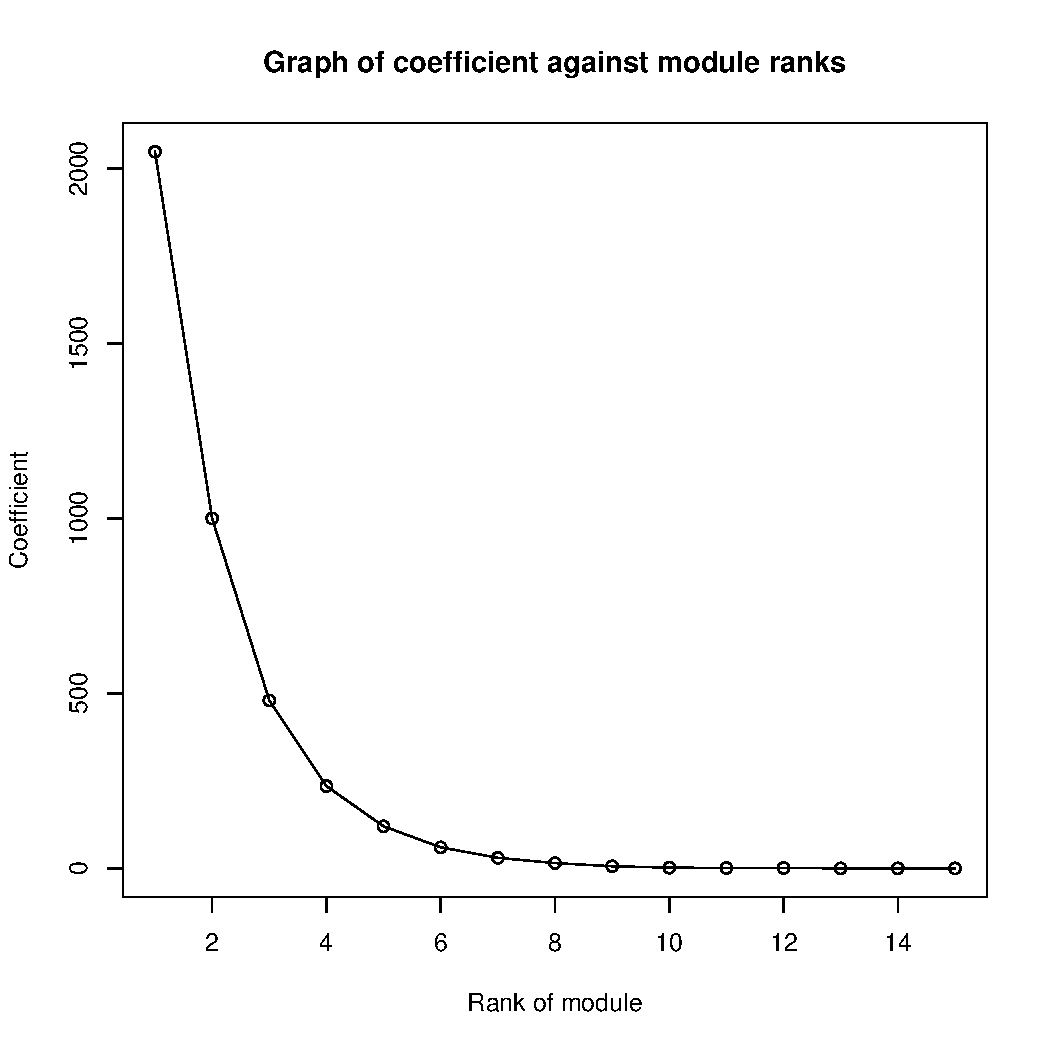
\includegraphics[width=0.6\linewidth]{images/gurobi_coefficients.pdf}}
  \end{center}
  \caption{Coefficients used in the solver's objective function}
  \label{gurobi_coeff}
\end{figure}

Figure~\ref{gurobi_coeff} shows a graph of the coefficients that were used in
the Gurobi-solved objective function. It demonstrates that the information
provided to the solver approximates the imaginary score function a staff
member might use.

To begin with, Gurobi's Python interface was used to prototype the model. As
the project implementer is more familiar with Python than with Java, it was
faster to prototype using the Python interface. Additionally, there is less
development overhead required with Python (i.e. no compilation necessary).

Once the Gurobi solver was working correctly on static data using the Python
interface, it was transferred to the application, changed to using the Java
interface and integrated with the application database.

A copy of the Gurobi code is included in Appendix~\ref{sec:gurobicode}.
